\chapter{实数的完备性}
\begin{introduction}
  \item 有理数的定义~\ref{def:rational-number}
  \item Bolzano-Weierstrass定理~\ref{theorem:Bolzano-Weierstrass}
  \item 数列极限的唯一性~\ref{theorem:limit-uniqueness}
  \item 数列极限的保序性逆命题~\ref{lemma:progression-order}

\end{introduction}
在本章中,我们将介绍实数的完备性。在介绍实数之前,我们需要将实数定义或者说引入。而对于实数的定义是有很多的,而我在此介绍无穷十进制小数表示和戴德金(Dedekind)分割。这部分我将结合陈纪修教授的教材和Ayumu的讲义。

在引入实数之前,我们需要先介绍有理数,而在介绍有理数之前,我们需要规定一些常用集合的记号。而介绍常用集合,则需要先介绍集合(set),在此我们并不介绍集合,我们暂时默认我们已经知道了集合的概念,将来我们会对该部分内容进行扩充。现在让我们来列举一些常用的集合。
\begin{definition}[常用集合表示]
$\mathbb{N} = \{ 1, 2, 3, \cdots, n, \cdots\}$

$\mathbb{Z} = \{ 0, \pm 1, \pm 2, \pm 3, \cdots, \pm n, \cdots \}$

$\mathbb{Z}^+ = \{ n | n \in \mathbb{Z}, n > 0 \}$
\end{definition}
在定义了以上的集合表示之后,我们就能以上的符号来表示有理数:
\begin{definition}[有理数] \label{def:rational-number} 
若一个数x可以表示成$\frac{q}{p}$的形式,其中$q \in \mathbb{Z}$, $p \in \mathbb{Z}^+$, 则称x为{\bf 有理数}(rational number)。而由有理数组成的集合称为{\bf 有理数集},有理数集常用$\mathbb{Q}$表示,其可以表示为:
\[ \mathbb{Q} = \{ x | x = \frac{q}{p}, q \in \mathbb{Z}, p \in \mathbb{Z}^+ \} \]
在这里, 我们可以看到p只需要属于$\mathbb{Z}^+$, 这是因为若x为负的, 我们总可以规定负号出现在分子上。
\end{definition}
有理数对加减乘除都封闭,并且我们在有理数上定义了大小关系,即有理数也是良序的。但是它并不能满足研究所需。例如,存在长度无法用有理数表示。并且有理数之间存在``空隙'',即有理数不连续。而在我们之后的研究中,我们往往需要研究连续性,因此我们需要对有理数进行扩充。在这之前,我们先来证明确实有一些数无法用有理数表示。


\begin{example}
$\sqrt{2}$不是有理数。
\end{example}
\begin{proof}
我们用反证法。假设$\sqrt{2}$为有理数, 那么存在$q \in \mathbb{Z}, p \in \mathbb{Z}^+$, $p, q$互质, 使得$\sqrt{2} = \frac{q}{p}$, 即$q^2 = 2p^2$。因为$q^2$可以被2整除, 即$q^2$为偶数, 则$q$为偶数。那么$q$可以表示为$q = 2m, m \in \mathbb{Z}$。代入上式中, 得$p^2 = 2m^2$, 即$p$也为偶数。这与互质矛盾, 因此假设不成立, $\sqrt{2}$不是有理数。
\end{proof}
\begin{example}
    若n不是完全平方数, 则$\sqrt{n}$不是有理数。
\end{example}
\begin{proof}
\end{proof}
除了以上举例的有些数无法用有理数表示以外, 有的函数在实数域和有理数域上的表现完全不一样,比如狄利克雷(dirichlet)函数:
\begin{equation*}
    D(x) = \left\{
        \begin{aligned}
            1 &\quad x\text{是有理数} \\
            0 &\quad x\text{是无理数}
        \end{aligned}
    \right.
\end{equation*}

% 陈老视频8
\begin{theorem}[确界存在定理---实数系连续性定理]
    非空有上界的数集必有上确界,非空有下界的数集必有下确界。
\end{theorem}
\begin{proof}
    
\end{proof}

% 陈老视频9
\section{数列极限}
\begin{definition}[数列极限的定义]
    对于数列$\{ a_n \}$, 存在一个实常数a, 对$\forall \epsilon > 0$, $\exists N \in \mathbb{Z}^+$,使得当$n > N$时,$|a_n-a| < \epsilon$成立,则称$\{ a_n \}${\bf 收敛}(convengent)于a或者$\{ a_n \}$的{\bf 极限}(limit)为a, 记作
    \[ \lim_{n \to \infty} a_n = a \text{\quad 或者 \quad}  a_n \to a(n \to +\infty)\]
    若不存在实数a, 满足上述性质, 则称数列$\{ a_n \}${\bf 发散}(divergent)。
\end{definition}
在这里定义邻域的概念:$a$的$\epsilon$邻域$O(a, \epsilon)$为:$(a-\epsilon, a+\epsilon)$。因此数列极限的定义也可以描述为: 当$n > N$时, $a_n$落在a的$\epsilon$邻域内。

并且,一个数列的极限还有以下的一些性质。首先, 一个数列是否收敛, 收敛的话, 收敛于哪个数, 这与数列的前有限项无关。这是因为, 假如数列收敛于A, 我对前K项做了修改, 那么$\forall \epsilon > 0$, 可以取$N' = \max\{K, N\}$, 此时$\left| x_n -A \right| < \epsilon$, 即极限依旧为A。又比如极限不存在时, 则$\exists \epsilon > 0$, $\forall N \in \mathbb{N}^+$, $\exists n > N$, $\left| x_n - A \right| > \epsilon$。此时, $\forall N > K$, $\exists n > N$, $\left| x_n -A \right| > \epsilon$, 那么$N < K$时也成立。因此在求极限的不等式时, 可以从选定的一个N开始,有时候会使得不等式的求解方便。

此外, $\epsilon$还可以限定为小于一定值, 在该限定下证明不等式成立。这是因为当$\epsilon \le c$时候, 存在了N, 使得$n > N$时成立, 那么当$\epsilon > c$时, 该N也能使得$n >N$时成立。

接下来我们定义一个特殊的数列极限: {\bf 无穷小量}。我们会在之后特殊讨论它, 例如无穷小量的阶。 
\begin{definition}[无穷小量的定义]
    以零为极限的变量称为{\bf 无穷小量}。
\end{definition}

\begin{example}
    证明:
    \[ \mylim{n}{\frac{n}{n+3}}= 1 \]
\end{example}
\begin{proof}
    令:
    \[ \left| \frac{n}{n+3} - 1 \right| = \frac{3}{n + 3} < \frac{3}{n} < \epsilon \]
    因此, 当$N = \left[ \frac{3}{\epsilon} \right] + 1$时, $\left| \frac{n}{n+3} - 1 \right| < \epsilon$
\end{proof}

\begin{example}
    证明:
    \[ \mylim{n}{q^n}= 0(0 < \left|q\right| < 1) \]
\end{example}
\begin{proof}
    因为$0< \left|q\right| < 1$, 则$\left|q^n\right| = \left|q\right|^n < \epsilon$, 则:
    \[ n > \frac{\lg(\epsilon)}{\lg(\left|q\right|)} \]
    因为$N \in \mathbb{N}^+$, 所以取$N = \max\left\{1, \left[ \frac{\lg(\epsilon)}{\lg(\left|q\right|)} \right]\right\}$, 当$n > N$时, $\left| q^n - 0 \right| < \epsilon$, 即:
    \[ \mylim{n}{q^n} = 0(0 < \left|q\right| < 1) \]
\end{proof}

% 陈老视频10
\begin{example}\label{example-chapter2-1}
    证明:
    \[ \lim_{n \to \infty } \sqrt[n]{a}= 1 (a > 1)\]
\end{example}
\begin{proof}
    因为$a > 1$, 所以$\left| \sqrt[n]{a} - 1 \right| =\sqrt[n]{a} - 1$:
    \begin{equation*}
        \sqrt[n]{a} - 1 = \sqrt[n]{1\cdot 1\cdot 1\cdots a} - 1 < \frac{(n - 1) + a}{n} - 1 < \frac{a - 1}{n} < \frac{a}{n} < \epsilon 
    \end{equation*}
    所以取$N = \left[ \frac{a}{\epsilon} \right] + 1$时, $\forall n > N$, $\left| \sqrt[n]{a} - 1\right| < \epsilon$, 即$\mylim{n}{\sqrt[n]{a}} = 1$。

    \framebox{陈老是这样证明的}:

    令$y_n = \sqrt[n]{a} - 1$, 则:
    \begin{equation*}
        a = (1 + y_n)^n = 1 + C_n^1 y_n + C_n^2 y_n^2 + \cdots + C_n^n y_n^n         
    \end{equation*}

    则:
    \[ 1 + ny_n < a \]
    即:
    \[ y_n < \frac{a - 1}{n} < \epsilon \]
    则取$N = \left[ \frac{a - 1}{\epsilon} \right] + 1$, , $\forall n > N$, $\left| \sqrt[n]{a} - 1\right| < \epsilon$, 即$\mylim{n}{\sqrt[n]{a}} = 1$
\end{proof}
\begin{remark}
    对于$\sqrt[n]{1+x}$利用均值不等式可以得到一个有意思的不等式:
    \begin{equation*}
        \sqrt[n]{1+x} < 1 + \frac{x}{n}
    \end{equation*}
\end{remark}
\begin{example}
    证明
    \[ \lim_{n \to \infty } \sqrt[n]{n}= 1 \]
\end{example}
\begin{proof}
    因为$n \ge 1$, 所以$\left| \sqrt[n]{n} - 1 \right| = \sqrt[n]{n} - 1$:
    \[ \sqrt[n]{n} -1 = \sqrt[n]{1\cdot 1\cdot 1\cdots \sqrt{n} \cdot \sqrt{n} } -1 < \frac{n-2+2\sqrt{n}}{n} - 1 < \frac{2}{\sqrt{n}} < \epsilon \]
    所以取$N = \left[ \frac{4}{\epsilon^2}\right] + 1$时, $\forall n > N$, $\left| \sqrt[n]{n} - 1\right| < \epsilon$, 即$\mylim{n}{\sqrt[n]{n}} = 1$。

    \framebox{陈老是这样证明的}:

    令$y_n = \sqrt[n]{n} - 1$, 则:
    \begin{equation*}
        n = (1 + y_n)^n = 1 + C_n^1 y_n + C_n^2 y_n^2 + \cdots + C_n^n y_n^n
    \end{equation*}
    则:
    \[ 1 + C_n^2 y_n^2 < n \]
    即
    \[ y_n < \sqrt{\frac{2}{n}} < \epsilon \]
    则取$N = \left[ \frac{2}{\epsilon^2} \right] + 1$, , $\forall n > N$, $\left| \sqrt[n]{n} - 1\right| < \epsilon$, 即$\mylim{n}{\sqrt[n]{n}} = 1$
\end{proof}

\begin{remark}
    实际上, 用以上两种方法, 我们可以证明$\mylim{n}{\sqrt[n]{n^k}} = 1, (k \in \mathbb{N}^+)$。
\end{remark}

\begin{example}
    证明:
    \[ \lim_{n \to \infty } \sqrt[n]{n^k}= 1, (k \in \mathbb{N}^+) \]
\end{example}
\begin{proof}
    因为$n \ge 1$, 所以$\left| \sqrt[n]{n^k} - 1 \right| = \sqrt[n]{n^k} - 1$:
    \[ \sqrt[n]{n} -1 = \sqrt[n]{1\cdot 1\cdot 1\cdots \sqrt{n} \cdot \sqrt{n} \cdot \sqrt{n} } -1 < \frac{n-2k+2k\sqrt{n}}{n} - 1 < \frac{2k}{\sqrt{n}} < \epsilon \]
    所以取$N = \left[ \frac{4k^2}{\epsilon^2}\right] + 1$时, $\forall n > N$, $\left| \sqrt[n]{n^k} - 1\right| < \epsilon$, 即$\mylim{n}{\sqrt[n]{n^k}} = 1$。

    \framebox{陈老证明方法}:
    取$n > 2k$, 令$y_n = \sqrt[n]{n^k} - 1$, 则:
    \begin{equation*}
        n^k = (1 + y_n)^n = 1 + C_n^1 y_n + \cdot + C_n^{k+1}y_n^{k+1} + \cdots + C_n^n y_n^n
    \end{equation*}
    则:
    \begin{equation*}
        \frac{(n-k)^{k+1}}{{(k+1)}^{k+1}}y_n^{k+1} < C_n^{k+1}y_n^{k+1} < n^k
    \end{equation*}
    则:
    \begin{equation*}
        y_n < (k+1)\sqrt[k+1]{\frac{n^k}{(n-k)^n(n-k)}}
    \end{equation*}
    因为$n > 2k$, 则$n-k = \frac{n}{2} + \frac{n}{2} - k > \frac{n}{2}$, 所以:
    \begin{equation*}
        yn < (k+1)\sqrt[k+1]{\frac{n^k}{(n-k)^n(n-k)}} < (k+1)\sqrt[k+1]{\frac{2^k}{(n-k)}} < \epsilon
    \end{equation*}
    则取:
    \begin{equation*}
        N = \max\left\{ 2k, \left[ \frac{2^k}{\left( \frac{\epsilon}{k+1} \right)^{k+1}}\right] + k + 1\right\}
    \end{equation*}
    当$n > N$时,$yn < \epsilon$, 即$\mylim{n}{\sqrt[n]{n^k}} = 1$
\end{proof}
\begin{remark}
    在知道极限的四则运算法则后, $\sqrt[n]{n^k} = \left(\sqrt[n]{n}\right)^k$可以很快得出极限为1。
\end{remark}


\begin{example}\label{example-chapter2-2}
    设$a_n > 0$,$\lim_{n \to \infty} a_n = a$,证明
    \begin{equation*}
        \mylim{n}{\mean{a}{n}} = a
    \end{equation*}
\end{example}
\begin{proof}
    \def\tmp#1{\left| a_{#1} - a \right|}
    \edef\tmpmax#1{\max\left\{#1\right\}}
    因为$\mylim{n}{a_n} = a$, 所以$\exists N \in \mathbb{N}^+$, $\forall n > N$, $\tmp{n} < \frac{\epsilon}{2}$。
    \begin{equation*}
        \begin{aligned}
            \left| \mean{a}{n} -a \right| &\le  \frac{\tmp{1} + \tmp{2} + \cdots + \tmp{n}}{n} \\
            & = \frac{\tmp{1} + \cdots + \tmp{N}}{n} + \frac{\tmp{N+1} + \cdots + \tmp{n}}{n} 
        \end{aligned}    
    \end{equation*}
    对于后一项, 当$n > N$时, 有:
    \begin{equation*}
        \frac{\tmp{N+1} + \cdots + \tmp{n}}{n} < \frac{n\epsilon/2}{n} < \frac{\epsilon}{2}
    \end{equation*}
    对于前一项, 因为N为一个有限数, 则取$M = \tmpmax{\tmp{1}, \tmp{2}, \cdots, \tmp{N}}$, 因此:
    \begin{equation*}
        \frac{\tmp{1} + \cdots + \tmp{N}}{n} < \frac{NM}{n}
    \end{equation*}
    因此取$N_1 = \left[ \frac{2NM}{\epsilon} + 1 \right]$, 当$n > N_1$时:
    \begin{equation*}
        \frac{\tmp{1} + \cdots + \tmp{N}}{n} < \frac{\epsilon}{2}
    \end{equation*}
    因此, 取$N_2 = \tmpmax{N, N_1}$, 当$n > N_2$时:
    \begin{equation*}
        \mean{a}{n} < \epsilon
    \end{equation*}
    即:
    \begin{equation*}
        \mylim{n}{\mean{a}{n}} = a
    \end{equation*}
\end{proof}

在给出数列极限的定义之后, 我们来考察下数列极限的性质。因为现在我们只讲了定义, 如果求所有的导数都从定义出发, 那么过程会极其地繁琐。因此我们需要总结规律, 使得我们能够方便地求解数列极限。
\begin{theorem}[数列极限的唯一性]\label{theorem:limit-uniqueness}
    若
    \begin{equation*}
        \mylim{n}{x_n} = a, \mylim{n}{x_n} = b
    \end{equation*}
    则
    \begin{equation*}
        a = b
    \end{equation*}
\end{theorem}
\begin{remark}
    以下我不再写$N \in \mathbb{N}^+$, 因为过于冗余。
\end{remark}
\begin{proof}
    \framebox{证法一(陈老版本)}: $\forall \epsilon > 0$, $\exists N_1$, $\forall n > N_1$, $\left| a_n - a \right|< \frac{\epsilon}{2}$。$\exists N_2$, $\forall n > N_2$, $\left| b_n - b \right|< \frac{\epsilon}{2}$。所以$\forall n > \max\{N_1, N_2\}$, 有:
    \begin{equation*}
        \left| a - b \right| = \left| (a - a_n) - (b - a_n) \right| \le \left| a_n - a \right| + \left| a_n - b \right| < \frac{\epsilon}{2} + \frac{\epsilon}{2} = \epsilon
    \end{equation*}
    即$\forall \epsilon$, $\forall n > \max\{N_1, N_2\}$, $\left| a - b \right| < \epsilon$。$\left| a - b \right| < \epsilon$要对所有的$\epsilon$和$n$都成立, 因此$\left| a - b \right| = 0$, 即$a = b$。若$a \neq b$, 则可取$\epsilon = \frac{\left| a - b \right|}{2}$, 使得$\exists n$使不等式不成立。

    \begin{remark}
        也可以把$\{a\}$看作一个恒等序列, 则$\forall \epsilon > 0$, $\exists N$, $\forall n > N$, $\left| a - b \right| < \epsilon$, 即恒等数列$\{a\}$的极限为b, 则$a = b$。
    \end{remark}

    \framebox{证法二}:用反证法, 设$a > b$, 取$\epsilon = \frac{a - b}{2}$, 则$\exists N_1$, $\forall n > N_1$, $\left| a_n - a \right| < \frac{a - b}{2}$, 则$a_n > \frac{a + b}{2}$。同理可得: $\exists N_2$, $\forall n > N_2$, $a_n < \frac{a + b}{2}$。则$\forall n > \max\{N_1, N_2\}$, $\frac{a+b}{2} < a_n < \frac{a+b}{2}$, 存在矛盾, 即$a \le b$。同理可以证$a \ge b$, 因此$a = b$。
\end{proof}
\begin{remark}
    唯一性表明了收敛的数列极限$a$有且只有一个, 在定义中只说了$\exists a$, 并没有限定$a$的个数, 唯一性使得当我们求得一个极限时, 不用再去找别的极限值。
\end{remark}

接下来我们再来看数列的有界性, 有界性也是极限非常重要的性质, 很多时候可以帮助我们放大不等式。

\begin{definition}\label{definition:limit-bound}
    \begin{enumerate}
        \item 对于数列$\collect{x_n}$, 若$\exists M \in \mathbb{R}$, $\forall n \in \mathbb{N}^+$, 成立$x_n \le M$, 则称M是$\collect{x_n}$的一个上界, 或称$\collect{x_n}$有上界。
        \item 对于数列$\collect{x_n}$, 若$\exists m \in \mathbb{R}$, $\forall n \in \mathbb{N}^+$, 成立$x_n \ge m$, 则称m是$\collect{x_n}$的一个下界, 或称$\collect{x_n}$有下界。
    \end{enumerate}
    $\collect{x_n}$既有上界又有下界, 则称$\collect{x_n}$有界。

    $\collect{x_n}$有界的另一个定义:$\exists X \in \mathbb{R}^+$, $\forall n \in \mathbb{N}^+$, 成立$\left| x_n \right| \le X$。
\end{definition}
\begin{remark}
    我们先说明下这两个定义等价: 若$\collect{x_n}$有上界有下界, 则$\forall n \in \mathbb{N}^+$, $m \le x_n \le M$, 则$\left| x_n \right| \le \max\left\{ |m|, |M|\right\}$, 则我们找到了$X = \max\left\{ |m|, |M|\right\}$。若$\collect{x_n}$有界,即$\exists X \in \mathbb{R}^+$, $\forall n \in \mathbb{N}^+$, $\left| x_n \right| \le X$, 则$\forall n \in \mathbb{N}^+$, $-X \le x_n \le X$, 则我们找到了$m = -X, M = X$。
\end{remark}

\begin{theorem}[数列极限的有界性]\label{theorem:limit-bound}
    若$\{ x_n \}$的极限存在,则$\{ x_n \}$有界。
\end{theorem}
\begin{proof}
    设$\collect{x_n}$的极限为$a$, 取$\epsilon = 1$, 则$\exists N$, $\forall n > N$, $\left| x_n - a \right| < 1$, 则$a - 1 < x_n < a + 1$。

    因为$N$是一个固定数, 则取$m = \min\{x_1, x_2, \cdots, x_N, a - 1\}$, $M = \max\{x_1, x_2, \cdots, x_N, a + 1\}$, $\forall n \in \mathbb{N}^+$, $m \le x_n \le M$。
\end{proof}
% 陈老视频11
\begin{theorem}[数列极限的保序性]\label{theorem:progression-order}
    存在两个数列$\{ x_n \}$和$\{ y_n \}$,并且
    \[ \mylim{n}{x_n} = a, \mylim{n}{y_n} = b, \text{\quad 且 \quad}a < b \]则$\exists N \in \mathbb{Z}^+$,当$n > N$时,$x_n < y_n$。
\end{theorem}
\begin{proof}
    取$\epsilon = \frac{b-a}{2}$, 则$\exists N_1$, $\forall a > N_1$, $\left| x_n - a \right| < \frac{b-a}{2}$, 即:
    \begin{equation*}
        x_n -a < \frac{b-a}{2} \rightarrow x_n < \frac{b+a}{2}
    \end{equation*}
    同理, $\exists N_2$, $\forall n > N_2$, $\left| y_n - b \right| < \frac{b-a}{2}$, 即:
    \begin{equation*}
        y_n - b > -\frac{b-a}{2} \rightarrow y_n > \frac{a+b}{2}
    \end{equation*}
    即$\forall n > \max\{N_1, N_2\}$, $x_n < \frac{a+b}{2} < y_n$。

    \qed
\end{proof}

\begin{lemma}[数列极限的保序性逆命题]\label{lemma:progression-order}
    对于$\mylim{n}{x_n} = a,\mylim{n}{x_n} = b$, 若$\exists N \in \mathbb{N}^+$, $\forall n > N$, $x_n \le y_n$, 则$a \le b$。 
\end{lemma}
\begin{proof}
    \framebox{反证法}: 若$a > b$, 则$\exists N_1$, $\forall n > N_1$, $x_n > y_n$, 则$\forall, n > \max\{N, N_1\}$, $x_n > y_n$, 这与$\forall n > N$, $x_n \le y_n$条件矛盾, 则假设不成立。

    \qed
\end{proof}
\begin{remark}
    \begin{enumerate}
        \item $\exists N$, $forall n > N$, $x_n < y_n$, 并不能推出$a < b$, 例如$\collect{x_n = \frac{1}{2n}}$和$\collect{y_n = \frac{1}{n}}$, 它们的极限都是0。
        \item 可以直接从极限存在的情况下的逆否命题的角度思考该命题。写出定理~\ref{theorem:progression-order}的逆否命题: 对于$\mylim{n}{x_n} = a,\mylim{n}{x_n} = b$, $\forall N$, $\exists n > N$, $x_n \ge y_n$, 则$a \ge b$, $\exists N$, $\forall n > N$, $x_n \ge y_n$满足该情况, 因此$a \ge b$。
    \end{enumerate}
\end{remark}

\begin{lemma}
    \begin{enumerate}
        \item 若$\mylim{n}{y_n} = b > 0$, 则$\exists N \in \mathbb{N}^+$, $\forall n > N$, $y_n > \frac{b}{2} > 0 $。
        \item 若$\mylim{n}{y_n} = b < 0$, 则$\exists N \in \mathbb{N}^+$, $\forall n > N$, $y_n < \frac{b}{2} < 0 $。
    \end{enumerate}
\end{lemma}
\begin{proof}
    利用数列极限的保序性证明。当$b > 0$时,取$\collect{x_n = \frac{b}{2}}$, 则$\mylim{n}{x_n} = \frac{b}{2} < b$, 由数列极限的保序性可知,$\exists N \in \mathbb{N}^+$, $\forall n > N$, 有$y_n > x_n = \frac{b}{2}$。 
    
    \qed

    同理可证明$b < 0$的情况。
\end{proof}
以上推论可以合起来写为:
\begin{lemma}\label{lemma:progression-order-b}
    若$\mylim{n}{y_n} = b \neq 0$, 则$\exists N \in \mathbb{N}^+$, $\forall n > N$, $\left| y_n \right|> \frac{\left| b \right|}{2} > 0 $。
\end{lemma}
\begin{proof}
    除了上一个推论那样分开来证明, 还可以如下证明:
    $\mylim{n}{y_n} = b$, 即$\forall \epsilon > 0$, $\exists N \in \mathbb{N}^+$, $\forall n > N$, $\left| y_n - b\right| < \epsilon$。

    由三角不等式得:
    \begin{equation*}
        \left| y_n - b\right| \ge \left| \left| y_n \right| - \left| b \right| \right|
    \end{equation*}
    即:
    \begin{equation*}
        \left| \left| y_n \right| - \left| b \right| \right| \le \left| y_n - b\right| < \epsilon
    \end{equation*}
    因此$\mylim{n}{\left| y_n \right|} = \left| b \right|$。之后的证明同上。
\end{proof}

\begin{theorem}[数列极限的夹逼性定理]
    对于数列$\collect{x_n}$, $\collect{y_n}$, $\collect{z_n}$, 若$\exists N \in \mathbb{N}^+$, $\forall n > N$, 成立$x_n \le y_n \le z_n$, 且$\mylim{n}{x_n} = \mylim{n}{z_n} = a$, 则$\mylim{n}{y_n} = a$
\end{theorem}
\begin{proof}
    $\forall \epsilon$, $\exists N_1 \in \mathbb{N}^+$, $\forall n > N_1$, $\left| x_n - a\right| < \epsilon$, 即$x_n -a > -\epsilon$。

    同理, $\forall \epsilon$, $\exists N_2 \in \mathbb{N}^+$, $\forall n > N_2$, $\left| y_n - a\right| < \epsilon$, 即$z_n -a < \epsilon$。

    取$N = \max\left\{ N_1, N_2 \right\}$, 则:
    \begin{equation*}
        -\epsilon < x_n - a < y_n - a < z_n - a < \epsilon
    \end{equation*}
    即: 
    \begin{equation*}
        -\epsilon < y_n - a <\epsilon
    \end{equation*}
    即:
    \begin{equation*}
        \left| y_n - a \right| < \epsilon
    \end{equation*}
    总结起来即为:
    $\forall \epsilon$, $\exists N \in \mathbb{N}^+$, $\forall n > N$, $\left| y_n - a\right| < \epsilon$, 即$\mylim{n}{y_n} = a$。

    \qed
\end{proof}
\begin{example}
    求: 
    \begin{equation*}
        \mylim{n}{\left(\sqrt{n+1} - \sqrt{n}\right)}
    \end{equation*}
\end{example}
\begin{proof}
    因为$\sqrt{n+1} > \sqrt{n}$, 所以$\sqrt{n+1} - \sqrt{n} > 0$。

    又因为:
    \begin{equation*}
        \sqrt{n+1}-\sqrt{n} = \frac{1}{\sqrt{n+1}+\sqrt{n}} < \frac{1}{2\sqrt{n}}
    \end{equation*}
    因此:
    \begin{equation*}
        0 < \sqrt{n+1} - \sqrt{n} < \frac{1}{2\sqrt{n}}
    \end{equation*}
    又因为$\mylim{n}{\frac{1}{2\sqrt{n}}} = 0$, 所以根据夹逼定理:
    \begin{equation*}
        \mylim{n}{\left(\sqrt{n+1}-\sqrt{n}\right)} = 0
    \end{equation*}
\end{proof}
\begin{example}
    证明:
    \begin{equation*}
        \mylim{n}{\left( a_1^n + a_2^n + \cdots + a_p^n \right)^\frac{1}{n}} = \max_{1 \le i \le p}\{a_i\}
    \end{equation*}
    其中$a_1, a_2, \cdots, a_p > 0$, 且为常数。
\end{example}
\begin{proof}
    \def\tmp{\left(a_1^n + a_2^n + \cdots + a_p^n\right)^{\frac{1}{n}}}
    设$M = \max_{1 \le i \le p}\{a_i\}$, 则
    \begin{equation*}
        \begin{aligned}
            \tmp > M \\
            \tmp \le p^{\frac{1}{n}}M 
        \end{aligned}
    \end{equation*}
    在之前的证明中我们已经证明$\mylim{n}{\sqrt[n]{p}} = 1$, 因此根据夹逼定理:
    \begin{equation*}
        \mylim{n}{\tmp} = M
    \end{equation*}

    \qed
\end{proof}

\begin{example}
    用夹逼定理证明:
    \begin{equation*}
        \mylim{n}{\sqrt[n]{n}} = 1
    \end{equation*}
\end{example}
\begin{proof}
    这个用夹逼定理的证明实际上和之前提到的方法1接近, 即利用
    \begin{equation*}
        \sqrt[n]{n} = \sqrt[n]{1\cdot1\cdot1\cdots\sqrt{n}\cdot\sqrt{n}} <\frac{n-2+2\sqrt{n}}{n} < \frac{2}{\sqrt{n}} + 1
    \end{equation*}
\end{proof}

\begin{example}
    用夹逼定理证明:
    \begin{equation*}
        \mylim{n}{\sqrt[n]{n^2}} = 1
    \end{equation*}
\end{example}
\begin{proof}
    这个用夹逼定理的证明实际上也和之前提到的方法1接近, 即利用
    \begin{equation*}
        \sqrt[n]{n^2} = \sqrt[n]{1\cdot1\cdot1\cdots\sqrt{n}\cdot\sqrt{n}\cdot\sqrt{n}\cdot\sqrt{n}} <\frac{n-4+4\sqrt{n}}{n} < \frac{4}{\sqrt{n}} + 1
    \end{equation*}
\end{proof}
% 陈老视频12
下面再来介绍下数列极限的四则运算, 有了四则运算法则我们可以快速地计算极限。推导四则运算法则需要用到数列极限的有界性。
\begin{theorem}[数列极限的四则运算]
    若$\lim\limits_{n \to \infty} x_n = a$, $\lim\limits_{n \to \infty} y_n = b$,则
    \begin{enumerate}
        \item $\mylim{n}{(\alpha x_n + \beta y_n)} = \alpha a + \beta b$
        \item $\mylim{n}{(x_n y_n)} = ab$
        \item $\mylim{n}{(\frac{x_n}{y_n})} = \frac{a}{b}(b \neq 0)$
    \end{enumerate}
\end{theorem}
\begin{proof}
    首先根据收敛数列的有界性有: $\exists X > 0$, $\left| y_n \right| \le X$。

    \begin{enumerate}
        \item 证明: $\mylim{n}{(\alpha x_n + \beta y_n)} = \alpha a + \beta$ b。
        
        $\forall \epsilon$, $\exists N_1$, $\forall n > N_1$, $\left| x_n - a \right| < \frac{\epsilon}{|\alpha|+|\beta|}$; $\forall \epsilon$, $\exists N_2$, $\forall n > N_2$, $\left| y_n - b \right| < \frac{\epsilon}{|\alpha|+|\beta|}$。

        则$\forall \epsilon$, $\exists N = \max\{N_1, N_2\}$, $forall n > N$, 有:
        \begin{equation*}
            \left| \alpha x_n + \beta y_n - \alpha a - \beta b\right| \le |\alpha||x_n-a| + |\beta||y_n-b| < \epsilon
        \end{equation*}
        即:
        \begin{equation*}
            \mylim{n}{(\alpha x_n + \beta y_n)} = \alpha a + \beta b
        \end{equation*}
        \qed
        \item 证明: $\mylim{n}{(x_n y_n)} = ab$
        
        \begin{equation*}
            | x_ny_n - ab | = |x_ny_n - ay_n +ay_n - ab| \le | x_n - a||y_n| + |a||y_n - b| \le X|x_n-a| +|a||y_n-b| 
        \end{equation*}
        $\forall \epsilon$, $\exists N_1, N_2$, $\forall n > N_1$, $|x_n - a| < \frac{\epsilon}{X+|a|}$, $\forall n > N_2$, $|y_n - b| < \frac{\epsilon}{X+|a|}$。则$\forall n > \max\{N_1, N_2\}$, 有
        \begin{equation*}
            | x_ny_n - ab | < \epsilon
        \end{equation*}
        即:
        \begin{equation*}
            \mylim{n}{(x_n y_n)} = ab
        \end{equation*}
        \qed
        \item 证明: $\mylim{n}{(\frac{x_n}{y_n})} = \frac{a}{b}(b \neq 0)$
        
        因为$\mylim{n}{y_n} = b \neq 0$, 根据引理~\ref{lemma:progression-order-b}: $\exists N_0$, $\forall n > N_0$, $|y_n| > \frac{|b|}{2} > 0$。则:
        \begin{equation*}
            \left|\frac{x_n}{y_n} - \frac{a}{b} \right| = \frac{|bx_n - ay_n|}{|b||y_n|} < \frac{2|bx_n-ab+ab-ay_n|}{|b|^2} \le \frac{2(|b||x_n-a|+|a||y_n-b|)}{|b|^2}
        \end{equation*}
        $\forall \epsilon$, $\exists N_1, N_2$, $\forall n > N_1$, $|x_n - a| < \frac{|b|^2\epsilon}{2(|a|+|b|)}$, $\forall n > N_2$, $|y_n - b| < \frac{|b|^2\epsilon}{2(|a|+|b|)}$。则$\forall n > \max\{N_0, N_1, N_2\}$:
        \begin{equation*}
            \left| \frac{x_n}{y_n} - \frac{a}{b} \right| < \epsilon
        \end{equation*}
        即:
        \begin{equation*}
            \mylim{n}{(\frac{x_n}{y_n})} = \frac{a}{b}
        \end{equation*}
        \qed
    \end{enumerate}
\end{proof}
\begin{remark}
    \begin{enumerate}
        \item 对于第三个式子, 我们还可以先证明$\mylim{n}{\frac{1}{y_n}} = \frac{1}{b}$, 再用第二个式子, 这样的方式简化运算。
        \item 四则运算的适用范围是极限存在, 发散的情况下则不适用了。
    \end{enumerate}
\end{remark}

\begin{example}
    求:
    \begin{equation*}
        \mylim{n}{\frac{5^{n+1}-(-2)^n}{3 \cdot 5^n + 2\cdot 3^n}} 
    \end{equation*}
\end{example}
\begin{proof}
    上下同除以$5^n$, 则:
    \begin{equation*}
        \frac{5^{n+1}-(-2)^n}{3 \cdot 5^n + 2\cdot 3^n} = \frac{5-\left(-\frac{2}{5}\right)^n}{3+2\left(\frac{3}{5}\right)^n}
    \end{equation*}
    根据极限的四则运算得:
    \begin{equation*}
        \mylim{n}{\frac{5^{n+1}-(-2)^n}{3 \cdot 5^n + 2\cdot 3^n}} = \frac{5}{3}
    \end{equation*}
\end{proof}

\begin{example}
    当$a > 0$时, 证明:
    \begin{equation*}
        \mylim{n}{\sqrt[n]{a}} = 1
    \end{equation*}
\end{example}
\begin{proof}
    在例题~\ref{example-chapter2-1}中我们已经证明了当$a > 1$时:
    \begin{equation*}
        \mylim{n}{\sqrt[n]{a}} = 1
    \end{equation*}
    当$a = 1$时, $\sqrt[n]{a} = 1$, 极限显然成立。

    当$a < 1$时:
    \begin{equation*}
        \sqrt[n]{a} = \frac{1}{\sqrt[n]{\frac{1}{a}}}
    \end{equation*}
    因为$a < 1$, 则$\frac{1}{a} > 1$, 则根据$a > 1$的情况得:
    \begin{equation*}
        \mylim{n}{\sqrt[n]{\frac{1}{a}}} = 1
    \end{equation*}
    根据极限的四则运算得:
    \begin{equation*}
        \mylim{n}{\sqrt[n]{a}} = 1
    \end{equation*}
    综上, $\mylim{n}{\sqrt[n]{a}} = 1$。

    \qed
\end{proof}

\begin{example}
    求:
    \begin{equation*}
        \mylim{n}{n\left( \sqrt{n^2+1} - \sqrt{n^2 - 1}\right)}
    \end{equation*}
\end{example}
\begin{proof}
    因为:
    \begin{equation*}
        n\left(\sqrt{n^2+1} - \sqrt{n^2 - 1}\right) = \frac{2n}{\sqrt{n^2+1}+\sqrt{n^2-1}}
    \end{equation*}
    所以:
    \begin{equation*}
        \frac{n}{\sqrt{n^2+1}} < n\left(\sqrt{n^2+1} - \sqrt{n^2 - 1}\right) < \frac{n}{\sqrt{n^2-1}}
    \end{equation*}
    又因为:
    \begin{equation*}
        \mylim{n}{\frac{n}{\sqrt{n^2+1}}} = \mylim{n}{\frac{1}{\sqrt{1+\left(\frac{1}{n}\right)^2}}} = 1
    \end{equation*}
    同理:
    \begin{equation*}
        \mylim{n}{\frac{n}{\sqrt{n^2-1}}} = 1
    \end{equation*}
    因此根据夹逼定理:
    \begin{equation*}
        \mylim{n}{n\left( \sqrt{n^2+1} - \sqrt{n^2 - 1}\right)} = 1
    \end{equation*}

    \framebox{陈老的证明}:
    \begin{equation*}
        n\left(\sqrt{n^2+1} - \sqrt{n^2 - 1}\right) = \frac{2n}{\sqrt{n^2+1}+\sqrt{n^2-1}} = \frac{2}{\sqrt{1+\left(\frac{1}{n}\right)^2}+\sqrt{1-\left(\frac{1}{n}\right)^2}}
    \end{equation*}
    之后直接进行四则运算。
\end{proof}
\begin{remark}
    如果直接对原式使用四则运算,则会得到$\infty \cdot 0$, 该极限无法计算, 因此需要对式子进行变形。
\end{remark}

\begin{example}
    求:
    \begin{equation*}
        \mylim{n}{\left( \frac{1}{\sqrt{n^2+1}} + \frac{1}{\sqrt{n^2 + 2}} + \cdots \frac{1}{\sqrt{n^2+n}} \right)}
    \end{equation*}

\end{example}
\begin{proof}
    为了书写方便, 我们令:
    \begin{equation*}
        y_n = \frac{1}{\sqrt{n^2+1}} + \frac{1}{\sqrt{n^2 + 2}} + \cdots \frac{1}{\sqrt{n^2+n}}
    \end{equation*}
    对每一项进行缩放, 则:
    \begin{equation*}
        \frac{n}{\sqrt{n^2+n}} < y_n < \frac{n}{n} = 1
    \end{equation*}
    又因为:
    \begin{equation*}
        \mylim{n}{\frac{n}{\sqrt{n^2+n}}} = \mylim{n}{\frac{1}{\sqrt{1+\frac{1}{n}}}} = 1
    \end{equation*}
    根据夹逼定理得:
    \begin{equation*}
        \mylim{n}{y_n} = 1
    \end{equation*}
\end{proof}
\begin{remark}
    在数列中有无穷多项时, 我们不能直接用四则运算对每一项进行极限之后加和, 特别是每一项都趋向于0的情况下。四则运算只适用于有限项的情况下, 对于无限项的情况要具体讨论。
\end{remark}

\begin{example}
    设$a_n > 0$, $\mylim{n}{a_n} = a$,证明:
    \begin{equation*}
        \mylim{n}{\sqrt[n]{a_1a_2\cdots a_n}} = a
    \end{equation*}
\end{example}
\begin{proof}
    若$a > 0$, 根据均值不等式有:
    \begin{equation*}
        \frac{n}{\frac{1}{a_1}+\frac{1}{a_2}+\cdots+\frac{1}{a_n}} \le \sqrt[n]{a_1a_2\cdots a_n} \le \mean{n}{a}
    \end{equation*}
    根据例题~\ref{example-chapter2-2}的结果, 我们已知当$\mylim{n}{a_n} = a$时, 有:
    \begin{equation*}
        \mylim{n}{\mean{a}{n}} = a
    \end{equation*}
    根据极限的四则运算, 当$\mylim{n}{a_n} = a$时, $\mylim{n}{\frac{1}{a_n}} = \frac{1}{a}$, 根据例题~\ref{example-chapter2-2}, 有:
    \begin{equation*}
        \mylim{n}{\frac{\frac{1}{a_1}+\frac{1}{a_2}+\cdots+\frac{1}{a_n}}{n}} = \frac{1}{a}
    \end{equation*}
    则根据夹逼定理:
    \begin{equation*}
        \mylim{n}{\sqrt[n]{a_1a_2\cdots a_n}} = a
    \end{equation*}

    若$a = 0$, 则:
    \begin{equation*}
        0 < \sqrt[n]{a_1a_2\cdots a_n} \le \mean{n}{a}
    \end{equation*}
    同上, 可以证明:
    \begin{equation*}
        \mylim{n}{\sqrt[n]{a_1a_2\cdots a_n}} = 0
    \end{equation*}
    综上所诉:
    \begin{equation*}
        \mylim{n}{\sqrt[n]{a_1a_2\cdots a_n}} = a \quad (a_n > 0)
    \end{equation*}    

    \qed
\end{proof}

\begin{proposition}
    若$\{ x_n \}$是无穷小量,$\{ y_n \}$有界($| y_n | \le X$),则$\{ x_n y_n \}$也是无穷小量。
\end{proposition}
\begin{proof}
    因为$\collect{x_n}$为无穷小量, 则$\forall \epsilon > 0$, $\exists N$, $\forall n > N$, $|x_n| < \frac{\epsilon}{X}$。由于$\collect{y_n}$有界, 即$|y_n| \le X$, 则$\forall n > N$, 有: 
    \begin{equation*}
        |x_ny_n| = |x_n||y_n| < \epsilon
    \end{equation*}
    即$\collect{x_ny_n}$也是无穷小量。

    \qed
\end{proof}

\section{无穷大量}
% 陈老视频13
除了上一节中介绍的数列收敛的情况外, 有时候我们还需要研究数列趋向于无穷的情况。对于极限存在的情况, 我们是说: $\forall \epsilon$, $\exists N$, $\forall n > N$, $|x_n - a| < \epsilon$, 即在$n > N$之后, 数列的点落在$\rho(a, \epsilon)$邻域内。而对于无穷大的情况, 我们需要适当修改定义, 因为我们的极限并不趋于一个具体的有限值, 也就无法给出该有限值的邻域。要研究无穷大量, 我们需要理解什么是无穷。 我们可以这样理解无穷: 无穷比任意一个有限值都要大。接下来我们给出无穷大量的定义:
\begin{definition}[无穷大量]
对于一个数列$\{ x_n \}$,若对于任意给定的$G > 0$, 可以找到正整数N, 使得当$n > N$时,$| x_n |> G$,则称数列$\{ x_n \}$是无穷大量,记为
\[ \lim_{n \to \infty } x_n = \infty \]
若对于该数列$\{ x_n \}$, $| x_n |> G$可以恒表示为$x_n > G$,则称数列$\{ x_n \}$是正无穷大量,记为$+\infty$。

若对于该数列$\{ x_n \}$, $| x_n |> G$可以恒表示为$x_n < -G$,则称数列$\{ x_n \}$是负无穷大量,记为$-\infty$。
\end{definition}

\begin{example}
    设$| q | > 1$,证明$\{ q^n \}$是无穷大量。 
\end{example}
\begin{proof}
    \framebox{证明一(陈老证明)}: 取$G > |q|$, 令:
    \begin{equation*}
        \left| q^n \right| > G
    \end{equation*}
    则:
    \begin{equation*}
        n > \frac{\lg{G}}{\lg{|q|}}
    \end{equation*}
    则$\forall G > 0$, 取$N = \max\left\{\left[\frac{\lg{G}}{\lg{|q|}}\right], 1\right\}$, 当$n > N$时, $\left| q^n \right| > G$, 即$\collect{q^n}$是无穷大量。

    \qed

    \framebox{证明二}:
    \begin{equation*}
        \left| q^n \right| = (1 + |q| - 1)^n > n(|q| - 1) > G
    \end{equation*}
    则$\forall G > 0$, 取$N = \max\left\{\left[\frac{G}{|q|-1}\right], 1\right\}$, 当$n > N$时, $\left| q^n \right| > G$, 即$\collect{q^n}$是无穷大量。

    \qed
\end{proof}

\begin{proposition}
    证明$\{ \frac{n^2-1}{n+5} \}$是无穷大量。 
\end{proposition}
\begin{proof}
    
\end{proof}

\begin{lemma}\label{lemma:inverse}
    若$x_n \neq 0$,则$\{ x_n \}$是无穷大量的充要条件是$\{ \frac{1}{x_n} \}$是无穷小量。    
\end{lemma}
\begin{proof}

\end{proof}

% 陈老视频14
\begin{lemma}
    设$\{ x_n \}$是无穷大量,$\{ y_n \}$满足$\exists N_0 \in \mathbb{Z}^+$, $\forall n > N_0$,有$| y_n | \ge \delta > 0$,则$\{ x_n y_n\}$也是无穷大量。
\end{lemma}
\begin{proof}
\end{proof}

\begin{lemma}
    设$\{ x_n \}$是无穷大量,$\{ y_n \}$极限存在,且$\lim\limits_{n \to \infty}y_n = b \ne 0$,则$\{ x_n y_n\}$与$\left\{ \frac{x_n}{y_n} \right\}$都是无穷大量。
\end{lemma}
\begin{proof}
\end{proof}

\begin{proposition}
    $\{ \frac{n}{\sin(n)}\}$和$\{ n \cdot \arctan(n)\}$是无穷大量。
\end{proposition}
\begin{proof}
\end{proof}

\begin{proposition}
    讨论极限
    \[ \lim_{n \to \infty} \frac{\listsum{a}{n}{k}}{\listsum{b}{n}{l}}\]
    其中$a_0, b_0 \ne 0$, $k, l \in \mathbb{Z}^+$
\end{proposition}
\begin{proof}
    从分子上提出$n^k$,分母上提出$n^l$次
\end{proof}
\subsection{无穷大的运算}
若$\mylim{n}{x_n} = +\infty$,则记$\collect{x_n}$为``+$\infty$''。

若$\mylim{n}{y_n} = +\infty$,则记$\collect{y_n}$为``+$\infty$''。

若$\mylim{n}{z_n} = \infty$,则记$\collect{z_n}$为``+$\infty$''。

若$\mylim{n}{w_n} = 0$,则记$\collect{z_n}$为``0''。
\begin{theorem}
    \begin{enumerate}
        \item $(+\infty) + (+\infty) = +\infty$
        \item $(+\infty) - (-\infty) = +\infty$
        \item $(+\infty) \pm (\text{有界量}) = +\infty$
        \item $(+\infty) \cdot (+\infty) = +\infty$
        \item $(+\infty) \cdot (-\infty) = -\infty$
    \end{enumerate}
\end{theorem}

\begin{definition}
    \begin{enumerate}
        \item $(+\infty) - (+\infty) = ?$
        \item $(+\infty) + (-\infty) = ?$
        \item $0 \cdot \infty = ?$
        \item $\frac{0}{0} = ?$
        \item $\frac{\infty}{\infty} = ?$
        \item $\cdots$
    \end{enumerate}
    上述情况称为``待定型''
\end{definition}
\begin{definition}
    若数列$\collect{x_n}$,有$x_n \le x_{n + 1}, \forall n \in \mathbb{N}^+$,则称数列$\collect{x_n}$单调增加,记为$\collect{x_n} \uparrow$。若有$x_n < x_{n + 1}$,则称数列$\collect{x_n}$严格单调增加,记为$\collect{x_n} \text{严格} \uparrow$。
    
    若数列$\collect{x_n}$,有$x_n \ge x_{n + 1}, \forall n \in \mathbb{N}^+$,则称数列$\collect{x_n}$单调减少,记为$\collect{x_n} \downarrow$。若有$x_n > x_{n + 1}$,则称数列$\collect{x_n}$严格单调减少,记为$\collect{x_n} \text{严格} \downarrow$。
\end{definition}

\begin{theorem}[Stolz定理]
    假设$\collect{y_n}$严格单调增加数列,且$\mylinelim{n}{y_n} = + \infty$。若
    \[ \mylim{n}{ \frac{x_n - x_{n-1}}{y_n - y_{n-1}} } = a(a\text{为有限数}, +\infty, -\infty) \]
    则
    \[ \mylim{n}{\frac{x_n}{y_n}} = a\]
    
\end{theorem}
\begin{proof}
\framebox{因为陈老的证明简洁明了, 我们先写陈老的证明}:

当a = 0时: 
因为$\mylim{n}{y_n} = +\infty$, 则$\exists N_1 \in \mathbb{N}^+$, $\forall n > N_1$, $y_n > 0$。

又因为$\mylim{n}{\frac{x_n - x_{n-1}}{y_n - y_{n-1}}} = a$, 则$\forall \epsilon > 0$, $\exists N_2 \in \mathbb{N}^+$, $\forall n > N_2$, $\left| \frac{x_n - x_{n-1}}{y_n - y_{n-1}} \right| < \frac{\epsilon}{2}$。

取$N_3 = \max\{N_1, N_2\}$, $\forall n > N_3$:
\[  \left| x_n - x_{n-1}\right| < \frac{\epsilon}{2}\left| y_n - y_{n-1} \right| \]
又因为$\collect{y_n}$严格单调增加, 则上式可以化为:
\[  \left| x_n - x_{n-1}\right| < \frac{\epsilon}{2} \left( y_n - y_{n-1} \right) \]
根据三角不等式:
\[ \left| x_n - x_{N_3} \right| \le \left| x_n - x_{n-1}\right| + \left| x_{n-1} - x_{n-2} \right| + \cdots + \left| x_{N_3+1} - x_{N_3}\right|\]
根据上两式, 我们可以得出:
\[ \left| x_n - x_{N_3} \right| < \frac{\epsilon}{2} \left( y_n - y_{N_3} \right) \]
两边同除以$y_n$得:
\[ \left| \frac{x_n}{y_n} - \frac{x_{N_3}}{y_n} \right| < \frac{\epsilon}{2}(1 - \frac{y_{N_3}}{y_n}) < \frac{\epsilon}{2}\]
则根据三角不等式:
\[ \left| \frac{x_n}{y_n} \right| < \frac{\epsilon}{2} + \left|\frac{x_{N_3}}{y_n}\right|\]
因为$\mylim{n}{y_n} = +\infty$, $\exists N_4 \in \mathbb{N}^+$, $\forall n > N_4$, $y_n > \frac{2\left| x_{N_3}\right|}{\epsilon}$

则可以取$N = \max\{N_3, N_4\}$, $\forall n > N_4$:
\[ \left| \frac{x_n}{y_n} \right| < \epsilon \]
则对于$a = 0$时:
\[ \mylim{n}{\frac{x_n}{y_n}} = 0\]

当$a \neq 0 $时:

取$z_n = x_n - ay_n$, 则
\[ \frac{z_n-z_{n-1}}{y_n-y_{n-1}} = \frac{x_n-x_{n-1}}{y_n-y_{n-1}} - a \]
因此:
\[ \mylim{n}{\frac{z_n-z_{n-1}}{y_n-y_{n-1}}} = \mylim{n}{\left(\frac{x_n-x_{n-1}}{y_n-y_{n-1}} - a\right)} = 0\]
根据以上证明的$a = 0$的情况可知:
\[\mylim{n}{\frac{z_n}{y_n}} = 0\]
又因为:
\[ \frac{x_n}{y_n} = \frac{z_n}{y_n} + a\]
所以当$a \neq 0$时:
\[ \mylim{n}{\frac{x_n}{y_n}} = a\]

当$a = +\infty$时:

因为$\mylim{n}{\frac{x_n-x_{n-1}}{y_n-y_{n-1}}} = +\infty$, 则$\exists N_1 \in \mathbb{N}^+$, $\forall n > N_1$, $\frac{x_n-x_{n-1}}{y_n-y_{n-1}} > 1$, 即:
\[ x_n - x_{n-1} > y_n - y_{n-1} \]
因为$\collect{y_n}$严格单调增加, 则
\[ x_n - x_{n-1} > y_n - y_{n-1}> 0 \]
即$\collect{x_n}${\bf 严格单调增加}。

同时, 同其他情况的证明, 我们有:
\[ x_n - x_N > y_n - y_N\]

又因为$\mylim{n}{y_n} = +\infty$, 则$\forall G > \max\{0, y_N - x_N\}$, $\exists N_2 \in \mathbb{N}^+$, $\forall n > N_2$, $y_n > 2G$。

则
\[ x_n > y_n - y_N + x_N > G \]
即$\mylim{n}{x_n} = +\infty$, $\collect{x_n}$趋向于$+\infty$。

此时考虑$\frac{y_n - y_{n-1}}{x_n - x_{n-1}}$, 因为$\mylim{n}{\frac{x_n-x_{n-1}}{y_n - y_{n-1}}} = +\infty$, 则$\mylim{n}{\frac{y_n - y_{n-1}}{x_n-x_{n-1}}} = 0$(引理~\ref{lemma:inverse})。根据$a = 0$的情况得:$\mylim{n}{\frac{y_n}{x_n}} = 0$, 因此$\mylim{n}{\frac{x_n}{y_n}} = \infty$, 即$\forall G > 0$, $\exists N_3 \in \mathbb{N}^+$, $\forall n > N_3$, $\left| \frac{x_n}{y_n} \right| > G$。

又因为$\mylim{n}{y_n} = +\infty$, 则$\exists N_4 \in \mathbb{N}^+$, $\forall n > N_4$, $y_n > 0$, 同理$\exists N_5 \in \mathbb{N}^+$, $\forall n > N_5$, $x_n > 0$。

则当$n > \max\{ N_4, N_5 \}$时, $\frac{x_n}{y_n} > 0$。

即$\forall G > 0$, $\exists N = \max\{ N_3, N_4, N_5 \} \in \mathbb{N}^+$, $\forall n > N$, $\frac{x_n}{y_n} > G$, 即$\mylim{n}{\frac{x_n}{y_n}} = +\infty$。$a = +\infty$时也成立。
同理, 也能证明$a = -\infty$的情况。


现在用定义证明:

当a为有限数时:

因为$\mylim{n}{\frac{x_n-x_{n-1}}{y_n-y_{n-1}}} = a$, 则$\forall \epsilon > 0$, $\exists N_1 \in \mathbb{N}^+$, $\forall n > N_1$, $\left| \frac{x_n - x_{n-1}}{y_n - y_{n-1}} - a\right| < \frac{\epsilon}{2}$。

又因为$\mylim{n}{y_n} = +\infty$, 则$\exists N_2 \in \mathbb{N}^+$, $\forall n > N_2$, $y_n > 0$。

则$\forall n > N_3 = \max\{N_1, N_2\}$, 结合三角不等式, 我们有:
\[ \frac{x_n}{y_n}-a < \frac{\epsilon}{2}\left(1 - \frac{y_{N_3}}{y_n}\right) + \frac{x_{N_3}-ay_{N_3}}{y_n} < \frac{\epsilon}{2} + \frac{x_{N_3}-ay_{N_3}}{y_n}\]

因为$\mylim{n}{y_n} = +\infty$, 所以$\mylim{n}{\frac{x_{N_3}-ay_{N_3}}{y_n}} = 0$, 即$\exists N_4 \in \mathbb{N}^+$, $\forall n > N_4$, $\left| \frac{x_{N_3}-ay_{N_3}}{y_n} \right| < \frac{\epsilon}{2}$。

即$\forall \epsilon > 0$, $\exists N_5 = \max\{N_3, N_4\}$, $\forall n > N_5$, $\frac{x_n}{y_n} - a < \epsilon$。

同理可以证明:$\forall n > N_5$, $\frac{x_n}{y_n} - a > -\epsilon$。因此$\mylim{n}{\frac{x_n}{y_n}} = a$。
\end{proof}
\begin{proposition}
    用Stolz定理证明, 若$\mylim{n}{a_n} = a$,则
    \[ \mylim{n}{\mean{a}{n}} = a \]
\end{proposition}
\begin{proof}
\end{proof}

\begin{proposition}
    \[ \text{求} \mylim{n}{\frac{1^k+2^k+\cdots+n^k}{n^{k+1}}} \]
\end{proposition}
\begin{proof}

\end{proof}

\begin{proposition}
    \[ \text{设}\mylim{n}{a_n} = a\text{,求}\mylim{n}{\frac{a_1+2a_2+3a_3+\cdots+na_n}{n^2}} \]    
\end{proposition}
\begin{proof}

\end{proof}

% 陈老视频15
\section{收敛准则}
收敛数列一定有界,但是收敛数列不一定有界。
\begin{enumerate}
    \item 那么有界数列加什么条件收敛?
    \item 有界数列不加条件的情况下,可以得到什么弱一些的结论?
\end{enumerate}
\begin{theorem}
    单调有界数列必定收敛。
\end{theorem}
\begin{proof}
不妨设$\collect{x_n}$单调增加,有上界。
\end{proof}
定理意义: 从定义证明时, 我们需要知道极限a, 相当于验证极限为a, 而当极限未知时, 则无法证明。而定理则从数列本身的性质出发, 不需要知道极限是多少。

\begin{lemma}
    若数列$\collect{x_n}$从第N项之后开始单调有界, 则数列$\collect{x_n}$依旧收敛。
\end{lemma}
\begin{proof}
    考虑$n \ge N$后的数组成的数列, 设$n_1 = n - N + 1$, 则$\collect{x_{n_1}}$单调有界。由于$\collect{x_{n_1}}(n_1 \ge 1)$单调有界, 则$\collect{x_{n_1}}(n_1 \ge 1)$收敛。即$\exists a$, $\forall \epsilon > 0$, $\exists N_1$, $\forall n_1 > N_1$, 有$\left| x_{n_1} - a\right| < \epsilon$。那么我们可以取$N_2 = N_1 + N - 1$, 此时$\forall \epsilon$, $\exists N_2 = N_1 + N - 1$, $\forall n > N_2$, 有$\left| x_n - a\right| < \epsilon$, 即数列$\collect{x_n}$极限存在。
\end{proof}
\begin{proposition}
    设$x_1 > 0$, $x_{n+1} = 1 + \frac{x_n}{1+x_n}, n = 1,2, 3, \cdots$,证明$\collect{x_n}$收敛,并求极限。
\end{proposition}
\begin{proof}

\end{proof}

\begin{proposition}
    设$ 0 < x_1 < 1$, $x_{n+1} = x_n(1 - x_n), n = 1,2, 3, \cdots$,证明$\collect{x_n}$收敛,并求极限。
\end{proposition}
\begin{proof}

\end{proof}

无穷小量的趋近速度。
\begin{proposition}
    \[ \text{对于上题的}\collect{x_n},\text{求极限,}\mylim{n}{nx_n}\]
\end{proposition}
\begin{proof}

\end{proof}

% 陈老视频16
\begin{proposition}
    $ x_1 = \sqrt{2}, x_{n+1} = \sqrt{3+2x_n}, n = 1, 2, 3, \cdots $,证明$\collect{x_n}$收敛,并求极限。
\end{proposition}
\begin{proof}

\end{proof}

兔子
\begin{proposition}[Fibonacci数列]
    $\collect{a_n}$为Fibonacci数列, 令$b_n = \frac{a_{n+1}}{a_n}$,讨论$\collect{b_n}$数列。
    
\end{proposition}
\begin{proof}

\end{proof}

% 陈老视频17
接下来我们来研究$\pi$和$e$

关于$\pi$:
\begin{proposition}
    证明$\collect{L_n = n\sin \left ( \frac{180^\circ}{n} \right )}$收敛。求圆的面积公式。
\end{proposition}
\begin{proof}
取$t = \frac{180^\circ}{n(n+1)}$, 当$n \ge 3$时, $nt \le 45^\circ$。且由三角公式得: 
\[ \tan (nt) = \frac{\tan[(n-1)t] + \tan(t)}{1 - \tan[(n-1)t]tan(t)} \]
由于$nt \le 45^\circ$, 则$tan(kt) < 1(k < n)$, 因此: 
\[ \tan (nt) = \frac{\tan[(n-1)t] + \tan(t)}{1 - \tan[(n-1)t]tan(t)} > \tan[(n-1)t] + \tan(t)\]
则:
\begin{gather*}
    \tan(nt) > \tan[(n-1)t] + \tan(t) \\ 
    \tan[(n-1)t] > \tan[(n-2)t] + \tan(t) \\
    \cdots \cdots
\end{gather*}
则: 
\[ \tan(nt) > n\tan(t)\]
现在来考虑$\sin[(n+1)t]$: 
\[
\begin{split}
    \sin[(n+1)t] &= \sin(nt)\cos(t) + \cos(nt)\sin(t) \\
                &= \sin(nt)\cos(t)\left[ 1 + \frac{\tan(t)}{\tan(nt)}\right] \\
                &< \sin(nt)\cos(t)\left[ 1 + \frac{1}{n} \right] \\
                & < \sin(nt)\frac{n+1}{n}
\end{split}
\]
即: 
\[ n\sin[(n+1)t] < (n+1)\sin(nt) \]
将$t = \frac{180^\circ}{n(n+1)}$代入得: 
\[ n\sin\left( \frac{180^\circ}{n}\right) < (n + 1)\sin\left( \frac{180^\circ}{n+1} \right)\]
即该数列单调增加。

考虑到单位圆的面积: 
\[ S' > n \sin\left( \frac{180^\circ}{n}\right) \cos\left( \frac{180^\circ}{n}\right) \]
并且单位圆的面积小于外接正方形的面积, 即: 
\[ n \sin\left( \frac{180^\circ}{n}\right) \cos\left( \frac{180^\circ}{n}\right) < S' < 4 \]
即: 
\[ n\sin\left( \frac{180^\circ}{n}\right) < \frac{4}{\cos\left( \frac{180^\circ}{n}\right)}\]
因为$n \ge 3$, 所以: 
\[ n\sin\left( \frac{180^\circ}{n}\right) < 8\]
因此数列$\collect{L_n = n\sin \left ( \frac{180^\circ}{n} \right )}$单调有界, 则该数列极限存在。

现在定义$\mylim{n}{n\sin \left ( \frac{180^\circ}{n} \right )} = \pi$。

再来考虑单位圆的面积$S'$, 设内接正多边形的面积为$S_1$, 外接正多边形的面积为$S_2$, 则$S_1(n) < S' < S_2(n)$。内接正多边形的面积为:
\[ S_1(n) = n \sin\left( \frac{180^\circ}{n}\right) \cos\left( \frac{180^\circ}{n}\right)\]
外接正多边形的面积为: 
\[ S_2(n) = n \tan\left( \frac{180^\circ}{n}\right)  = n \frac{\sin\left( \frac{180^\circ}{n}\right)}{\cos\left( \frac{180^\circ}{n}\right)} \]
并且根据数列极限的四则运算有:
\[ \mylim{n}{S_1(n)} = \mylim{n}{n \sin\left( \frac{180^\circ}{n}\right)} \mylim{n}{\cos\left( \frac{180^\circ}{n}\right)} = \pi\]
\[ \mylim{n}{S_2(n)} = \frac{\mylim{n}{n\sin\left( \frac{180^\circ}{n}\right)}}{\mylim{n}{\cos\left( \frac{180^\circ}{n}\right)}} = \pi\]
则根据夹逼性定理得:
\[ S' = \pi \]

其中, 对于外接正多边形的面积, 考虑:
\[
\begin{split}
    (n+1)\tan(nt) - n \tan[(n+1)t] &= (n+1)\frac{\sin(nt)}{\cos(nt)} - n\frac{\sin[(n+1)t]}{\cos[(n+1)t]} \\
                        &= \frac{(n+1)\sin(nt)\cos[(n+1)t]-n\sin[(n+1)t]\cos(nt)}{\cos(nt)\cos[(n+1)t]} \\
                        &= \frac{\sin(nt)\cos[(n+1)t]-n\sin(t)}{\cos(nt)\cos[(n+1)t]} \\
                        &=\frac{\sin[(2n+1)t] - \sin(t) -2n\sin(t)}{2\cos(nt)\cos[(n+1)t]} \\
                        &= \frac{\sin[(2n+1)t] - (2n+1)\sin(t)}{2\cos(nt)\cos[(n+1)t]}
\end{split}
\]
并且当$n \ge 3$时, 有: 
\begin{gather*}
    \sin[(2n+1)t] = \sin(2nt)\cos(t) + \cos(2nt)\sin(t) < \sin(2nt) + \sin(t) \\
    \sin(2nt) = \sin[(2n-1)t]\cos(t) + \cos[(2n-1)t]\sin(t)  < \sin[(2n-1)t] + \sin(t)\\
    \cdots \cdots
\end{gather*}
因此: 
\[ sin[(2n+1)t] < (2n+1)\sin(t) \]
因此: 
\[ (n+1)\tan(nt) < n\tan[(n+1)t]\]
即:
\[ (n+1)\tan\left( \frac{180^\circ}{n+1}\right) < n\tan\left( \frac{180^\circ}{n}\right) \]
因此数列$\collect{n\tan\left( \frac{180^\circ}{n}\right)}$单调递减。因为外接正多边形面积必然大于内接正方形, 因此: 
\[ n\tan\left( \frac{180^\circ}{n}\right) > 2 \]
因此数列$\collect{n\tan\left( \frac{180^\circ}{n}\right)}$单调有界, 则该数列极限存在。

% 我们再用其他办法证明$\collect{L_n = n\sin \left ( \frac{180^\circ}{n} \right )}$有界: 

\end{proof}

关于$e$:
\begin{proposition}
    考虑两个数列:
    \[ \collect{x_n = \left(1 + \frac{1}{n}\right)^n} \quad \text{和} \quad \collect{y_n = \left(1 + \frac{1}{n}\right)^{n+1}} \]
    证明这两个数列极限存在且相等。
\end{proposition}
\begin{proof}
因为
\begin{equation*}
    \frac{n}{\frac{1}{a_1}+\frac{1}{a_2}+\cdots+\frac{1}{a_2}} \le \sqrt[n]{a_1a_2\cdots a_n}
\end{equation*}
所以:
\begin{equation*}
    \left( 1 + \frac{1}{n}\right)^{n+1} = 1\cdot\left( 1 + \frac{1}{n}\right)^{n+1} < \left(\frac{n+2}{1+(n+1)\cdot\frac{1}{1+\frac{1}{n}}}\right)^{n+2} = \left(\frac{n+2}{n+1}\right)^{n+2} = \left(1 + \frac{1}{n+1}\right)^{n+2}
\end{equation*}
所以$\collect{y_n = \left(1 + \frac{1}{n}\right)^{n+1}}$单调递减。
\end{proof}

定义$\ln = \log_e$为自然对数,$e$自然对数的底数。

\begin{proposition}
    令$a_n = 1 + \frac{1}{2^p} + \frac{1}{3^p} + \cdots + \frac{1}{n^p}, (p > 0)$,证明$\collect{a_n}$当$p>1$时收敛,当$p \le 1$时发散。    
\end{proposition}
\begin{proof}

$p = 1$时,$a_n = 1 + \frac{1}{2} +\frac{1}{3} + \cdots + \frac{1}{n}$为调和级数,它是正无穷大量,我们想知道它趋近无限的速度。
\end{proof}

% 陈老视频18
\begin{proposition}
证明
    \[ b_n = \left( 1 +\frac{1}{2} + \frac{1}{3} + \cdot + \frac{1}{n} \right) - \ln n \]
    收敛。
\end{proposition}
\begin{proof}
    极限记为$\gamma$,称为欧拉常熟。$\gamma >= 0.577215$
\end{proof}

\begin{proposition}
证明
\[ \mylim{n}{\frac{1}{n+1} + \frac{1}{n+2} + \cdots + \frac{1}{2n}} = \ln 2\]
\end{proposition}
\begin{proof}
除了夹逼定理,还能用上一个数列相减计算。
\end{proof}

\begin{proposition}
\[ d_n = 1- \frac{1}{2} + \frac{1}{3} - \frac{1}{4} + \cdots +(-1)^{n+}\frac{1}{n} \]
\end{proposition}
\begin{proof}

\end{proof}
以上是与$e$相关的数列

\begin{definition}[闭区间套]
    有一列闭区间$\collect{\left[a_n, b_n \right]}$,满足:
    \begin{enumerate}
        \item $\left[ a_{n+1}, b_{n+1}\right] \subset \left[ a_n, b_n\right], n = 1, 2, 3, \cdots $
        \item $b_n - a_n \to 0(n \to \infty)$
    \end{enumerate}
    则称这样的一列闭区间是一个闭区间套。
\end{definition}
\begin{theorem}[闭区间套定理]
    假如$\left[ a_n, b_n\right]$是一个闭区间套,则存在唯一的实数$\xi$,它属于一切闭区间$\left[ a_n, b_n\right]$。且$\mylim{n}{a_n} = \mylim{n}{b_n} = \xi$。
\end{theorem}
\begin{proof}
\end{proof}

\begin{theorem}
    实数集不可列。
\end{theorem}
\begin{proof}
    反证法
\end{proof}

% 陈老视频19
子列
\begin{definition}
    存在一个数列$\collect{x_n}$,取一列严格单调增加的正整数$n_1 < n_2 < n_3 < \cdots < n_k < \cdots$,则$x_{n_1}, x_{n_2}, \cdots, x_{n_k}, \cdot$称为$\collect{x_n}$的一个子列,记为$\collect{x_{n_k}}$, $k$代表子列中的第$k$项,又恰好是$\collect{x_n}$中的第$n_k$项。
\end{definition}
其中$n_k \ge k, \forall k$, $n_j > n_k, \forall j > k$。
\begin{theorem}
    设$\collect{x_n}$收敛于a, 则它的任何一个子列也收敛于a。即$\mylim{n}{x_n} = a$,证明$\mylim{k}{a_{n_k}} = a$
\end{theorem}
\begin{proof}

\end{proof}
可以用于证明数列不收敛。
\begin{proposition}
    若$\collect{x_n}$存在两个子列收敛于不同的极限,则$\collect{x_n}$发散。
\end{proposition}
\begin{proof}

\end{proof}

\begin{theorem}[Bolzano-Weierstrass定理]\label{theorem:Bolzano-Weierstrass}
    有界数列必有收敛子列。
\end{theorem}
\begin{proof}
    设数列为$\collect{x_n}$, 因为数列有界, 所以$\forall n >0$, 存在$a \le x_n \le b$, 则取$[a_1, b_1] = [a, b]$。

    将$[a_1, b_1]$分为两个闭区间, 分别为$[a_1, \frac{a_1+b_1}{2}]$和$[\frac{a_1+b_1}{2}, b_1]$, 其中至少有一个区间包含无穷多个数列的元素, 因为若两个区间都有有限个数列元素, 则数列$\collect{x_n}$的元素有限。那么我们可以取包含无穷多个数列元素的区间为$[a_2, b_2]$。

    同理, 我们可以取出$[a_3, b_3]$, $[a_4, b_4], \cdots$。每一个区间中都包含无穷多个数列元素。

    对于这些区间, $\forall n > 0, (1). [a_{n+1}, b_{n+1}] \subset [a_n, b_n]$, $(2). \mylim{n}{(b_n-a_n)} = \mylim{n}{\frac{b - a}{2^{n-1}}} = 0$, 则这些闭区间组成了一个闭区间套。根据闭区间套定理, 存在唯一的实数$\gamma$属于一切闭区间$[a_n, b_n]$。

    则我们可以这样构造子列: 
    
    从$[a_1, b_1]$中取$x_{n_1}$, 使得$n_1 > 0$, 这必然可以实现, 因为$[a_1, b_1]$中有无限多个数列元素。

    从$[a_2, b_2]$中取$x_{n_2}$, 使得$n_2 > n_1$, 这必然可以实现, 因为$[a_2, b_2]$中有无限多个数列元素, 即$\forall n_1, \exists n_2 > n_1$。

    从$[a_3, b_3]$中取$x_{n_3}$, 使得$n_3 > n_2$, 这必然可以实现, 因为$[a_3, b_3]$中有无限多个数列元素, 即$\forall n_2, \exists n_3 > n_2$。
    \[ \cdots \cdots \]

    对于子列$\collect{x_{n_k}}$, $x_{n_k} \in [a_k, b_k]$, 则$\forall \epsilon > 0 $, 取$K = \max\left\{\left[\log_2\left(\frac{b-a}{\epsilon}\right)\right] + 2, 1\right\}$, $\forall k > K, b_k - a_k < \epsilon $, 同时$x_{n_k} \in [a_k, b_k]$, $\gamma \in [a_k, b_k]$, 则$\forall k > K, \left| x_{n_k} - \gamma \right| < b_k - a_k < \epsilon$。

    即$\forall \epsilon > 0$, $\exists K \in \mathbb{N}^+$, $\forall k > K$, $\left| a_{n_k} - \gamma \right| < \epsilon$, 则$\mylim{k}{x_{n_k}} = \gamma$, 该子列收敛于$\gamma$。

    在陈老的视频是,陈老是用夹逼性证明$\collect{x_{n_k}}$收敛于$\gamma$, 证明如下: 
    
    $\forall k$, $a_k \le x_{n_k} \le b_k$, 且$\mylim{k}{a_k} = \mylim{k}{b_k} = \gamma$, 则根据夹逼性, $\mylim{k}{x_{n_k}} = \gamma$。{\bf 非常巧妙!}
\end{proof}

\begin{theorem}
    假设$\collect{x_n}$是无界数列,则存在子列$\collect{x_{n_k}}$,它是无穷大量。
\end{theorem}
\begin{proof}
    
\end{proof}

% 陈老视频20
Cauchy收敛原理

\begin{definition}
    $\collect{x_n}$满足:
    \[\forall \xi > 0, \exists N, \forall n, m > N, \left|x_n - x_m\right| < \xi \]
    则称$\collect{x_n}$为基本数列。
\end{definition}
也可以是$\forall m > n > N$
\begin{proof}
\end{proof}

\begin{proposition}
    判断
    \[ x_n = 1 + \frac{1}{2^2} + \frac{1}{3^2} + \cdots + \frac{1}{n^2} \]
    是否为基本数列。
\end{proposition}
\begin{proof}

\end{proof}

\begin{proposition}
    判断
    \[ x_n = 1 + \frac{1}{2} + \frac{1}{3} + \cdots + \frac{1}{n} \]
    是否为基本数列。
\end{proposition}
\begin{proof}

\end{proof}

\begin{theorem}[Cauchy收敛原理]
    $\collect{x_n}$收敛的充分必要条件是$\collect{x_n}$是基本数列。
\end{theorem}
\begin{proof}
{\bf 必要性}: 即$\collect{x_n}$收敛 $\Rightarrow$ $\collect{x_n}$是基本数列。

假设$\collect{x_n}$收敛于A, 则$\forall \epsilon > 0$, $\exists N \in \mathbb{N}^+$, $\forall n > N$, $\left| x_n - A \right| < \frac{\epsilon}{2}$。

则对于$\forall n, m > N$, $\left| x_n - x_m \right| < \left| x_n - A \right| + \left| x_m - A \right| < \frac{\epsilon}{2} + \frac{\epsilon}{2} = \epsilon $, 则$\collect{x_n}$为基本数列。

{\bf 充分性}: 即$\collect{x_n}$是基本数列$\Rightarrow$ $\collect{x_n}$收敛。

因为$\collect{x_n}$为基本数列, 即对于$\forall \epsilon > 0$, $\exists N \in \mathbb{N}^+$, $\forall m, n > N$, $\left| x_m - x_n \right| < \epsilon$。取$m = N + 1$, 则$\forall n > N$, $\left| x_{N+1} - x_n \right| < \epsilon$, 即$x_{N+1} -\epsilon < x_n < x_{N+1} + \epsilon $。则我们可以取$a = \min\left\{ x_1, x_2, \cdots, x_N, x_{N+1} - \epsilon \right\}, b = \max\left\{ x_1, x_2, \cdots, x_N, x_{N+1} + \epsilon \right\}$, 此时$\forall n \in \mathbb{N}^+$:
\[ a \le x_n \le b\]
即, $\collect{x_n}$数列有界。

根据Bolzano-Weierstrass定理(定理~\ref{theorem:Bolzano-Weierstrass}), 则存在收敛子列$\collect{x_{n_k}}$, 假设该收敛子列$\collect{x_{n_k}}$收敛于A, 则$\forall \epsilon > 0$, $\exists K \in \mathbb{N}^+$, $\forall k > K$, $\left| x_{n_k} - A \right| < \frac{\epsilon}{2}$, 又由于$\collect{x_n}$为基本数列, 则$\forall \epsilon > 0$, $\exists N' \in \mathbb{N}^+$, $\forall m', n' > N'$, $\left| x_{N+1} - x_{n'} \right| < \frac{\epsilon}{2}$。

取$N'' = \max\left\{N', n_K\right\}$, 因为$\collect{x_{n_{k'}}}$由无穷多项, 则必然存在$n_{k'} > N'' \ge n_K$, 即$k' > K$,。此时,因为$n_{k'} > N'' \ge N'$, 则$\forall n' > N'$, $\left| x_{n'} - x_{n_{k'}}\right| < \frac{\epsilon}{2}$, 又因为$k' > K$, 则$\left| x_{n_{k'}} - A\right| < \frac{\epsilon}{2}$, 因此$\forall n' > N'$, $\left| x_{n'} - A \right| < \left| x_{n'} - x_{n_{k'}} \right| + \left| x_{n_{k'}} - A \right| < \epsilon $, 即数列$\collect{x_n}$收敛。

而陈老是这样证明充分性的:

取$\epsilon = 1$, 因为$\collect{x_n}$是基本数列, 则$\exists N \in \mathbb{N}^+$, $\forall n > N$, $\left| x_n - x_{N+1} \right| < 1$, 因此$\left| x_n \right| < \left| x_n - x_{N+1} \right| + \left| x_{N+1} \right| < \left| x_{N+1} \right| + 1$。取$M = \max\left\{\left| x_1 \right|,\left| x_1 \right|,\cdots,\left| x_{N} \right|, \left| x_{N+1} \right| + 1\right\}
$, 则:
\[ \forall n \in \mathbb{N}^+, \left| x_n \right| \le M \]
即$\collect{x_n}$有界。

根据根据Bolzano-Weierstrass定理(定理~\ref{theorem:Bolzano-Weierstrass}), 则存在收敛子列$\collect{x_{n_k}}$, 假设该收敛子列$\collect{x_{n_k}}$收敛于A。

根据$\collect{x_n}$是基本数列, 则$\forall \epsilon > 0$, $\exists N_1 \in \mathbb{N}^+$, $\forall n, m > N_1$, $\left| x_n - x_m \right| < \frac{\epsilon}{2}$, 现在固定$x_m$, 取$x_n$为子列$\collect{x_{n_k}}$。现在考虑数列$\collect{\left| x_{n_k}  - x_m\right|}$和数列$\collect{\frac{\epsilon}{2}}$, 取$K = N_1$, 则$\forall k > K$, 有$n_k > n_K \ge K = N_1$, 即$\forall k > K$, $\left| x_{n_k}  - x_m\right| < \frac{\epsilon}{2}$, 根据数列极限的保序性逆命题(推论~\ref{lemma:progression-order}), $\left| A - x_m\right| \le \frac{\epsilon}{2} < \epsilon$。这对于$\forall m > N_1$都成立, 即数列$\collect{x_n}$极限存在且为A。
\end{proof}

\begin{proposition}
    $\collect{x_n}$满足压缩性条件,即
    \[ \left| x_{n+1} -x_n \right| \le k\left| x_n - x_{n-1}\right|, 0 < k < 1, \forall n = 2, 3, \cdots \] 
    则$\collect{x_n}$是收敛的。
\end{proposition}
\begin{proof}

\end{proof}

% 陈老视频21
实数系的基本定理
\begin{enumerate}
    \item 确界存在定理(实数系的连续性定理)
    \item 单调有界数列收敛定理
    \item 闭区间套定理
    \item Bolzano-Weierstrass定理
    \item Cauchy收敛原理(实数系完备性)
\end{enumerate}
以上都是在实数系中考虑, 实数系上的基本数列必然是收敛数列, 因此Cauchy收敛原理也被称为实数系的完备性定理。实数系有完备性, 有理数不具备完备性。例如$\collect{\left( 1 + \frac{1}{n}\right)^n}$是有理数列, 但是它的极限是无理数。以上五个定理等价。我们需要证明这五个定理等价。从Cauchy收敛原理推出闭区间套定理, 再从闭区间套定理推出确界存在定理。
\begin{theorem}
    实数系的完备性等价于实数系的连续性。
\end{theorem}
\begin{proof}
    (1)Cauchy收敛原理$\Rightarrow$闭区间套定理。

    (2)闭区间套定理$\Rightarrow$确界存在定理。
\end{proof}
\begin{figure}[htbp]
    \centering
    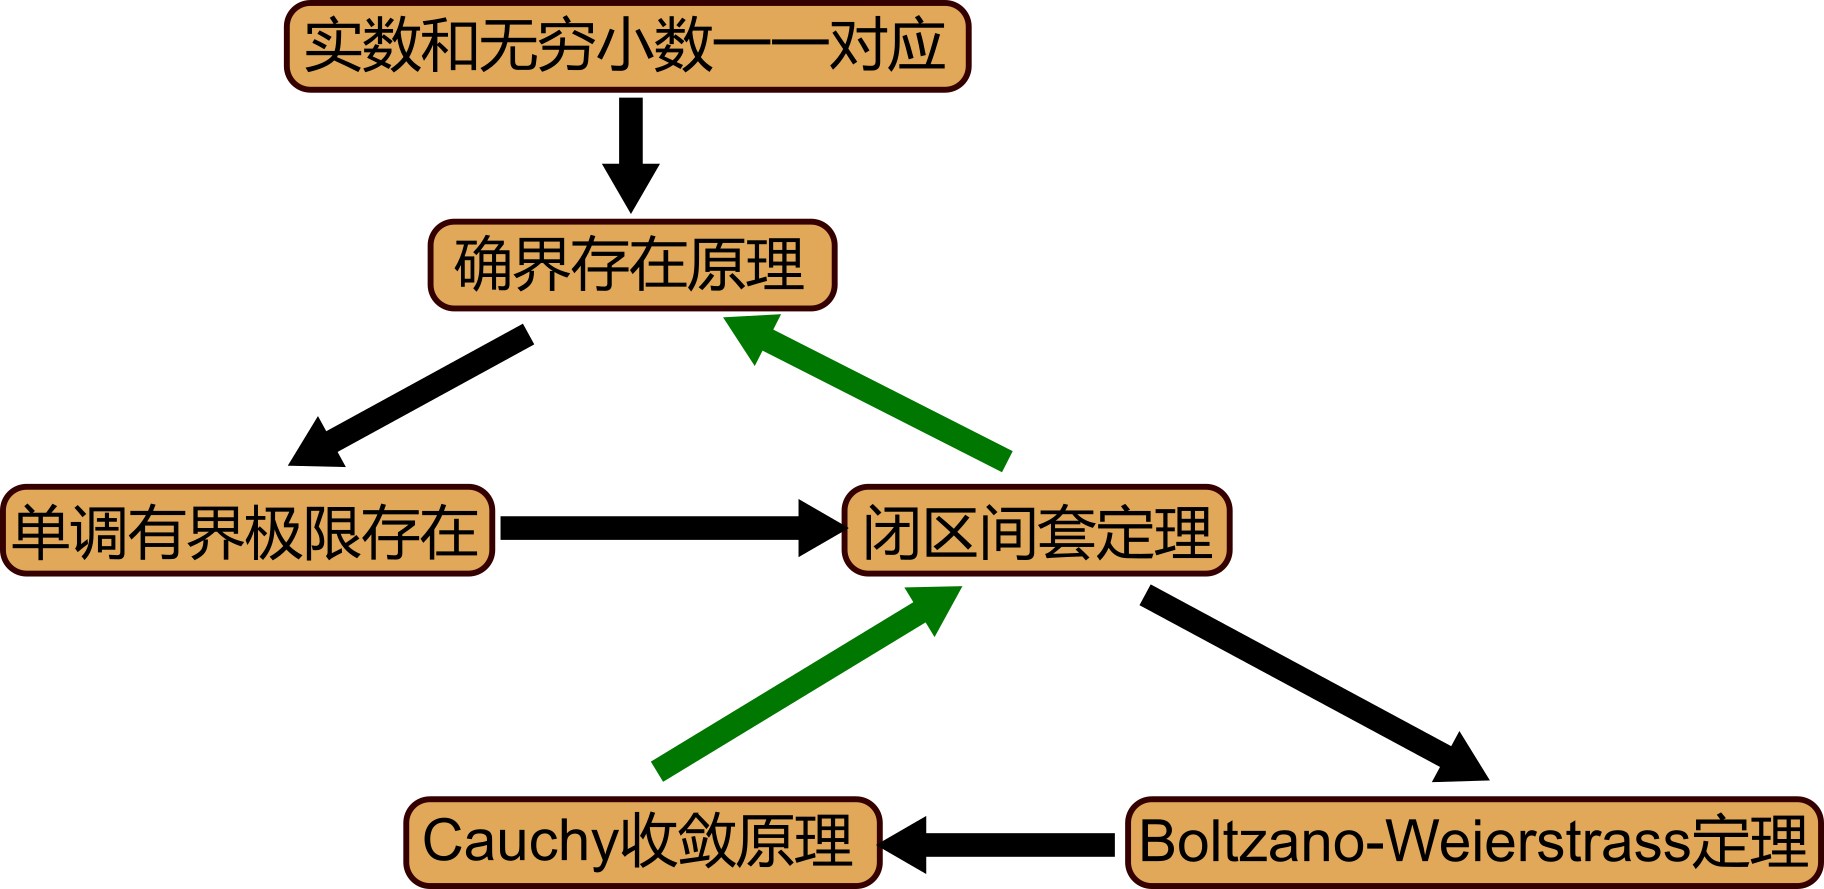
\includegraphics[width=0.7\linewidth]{theorem-relation.png}
    \caption{陈老视频中, 实数系定理的关系}
\end{figure}